\section{Evaluation}\label{sec:eval}

\subsection{Aggregated Nonblocking Communication}


\begin{figure}[tbh]
  \begin{center}
  % trimはleft bottom right topの順
  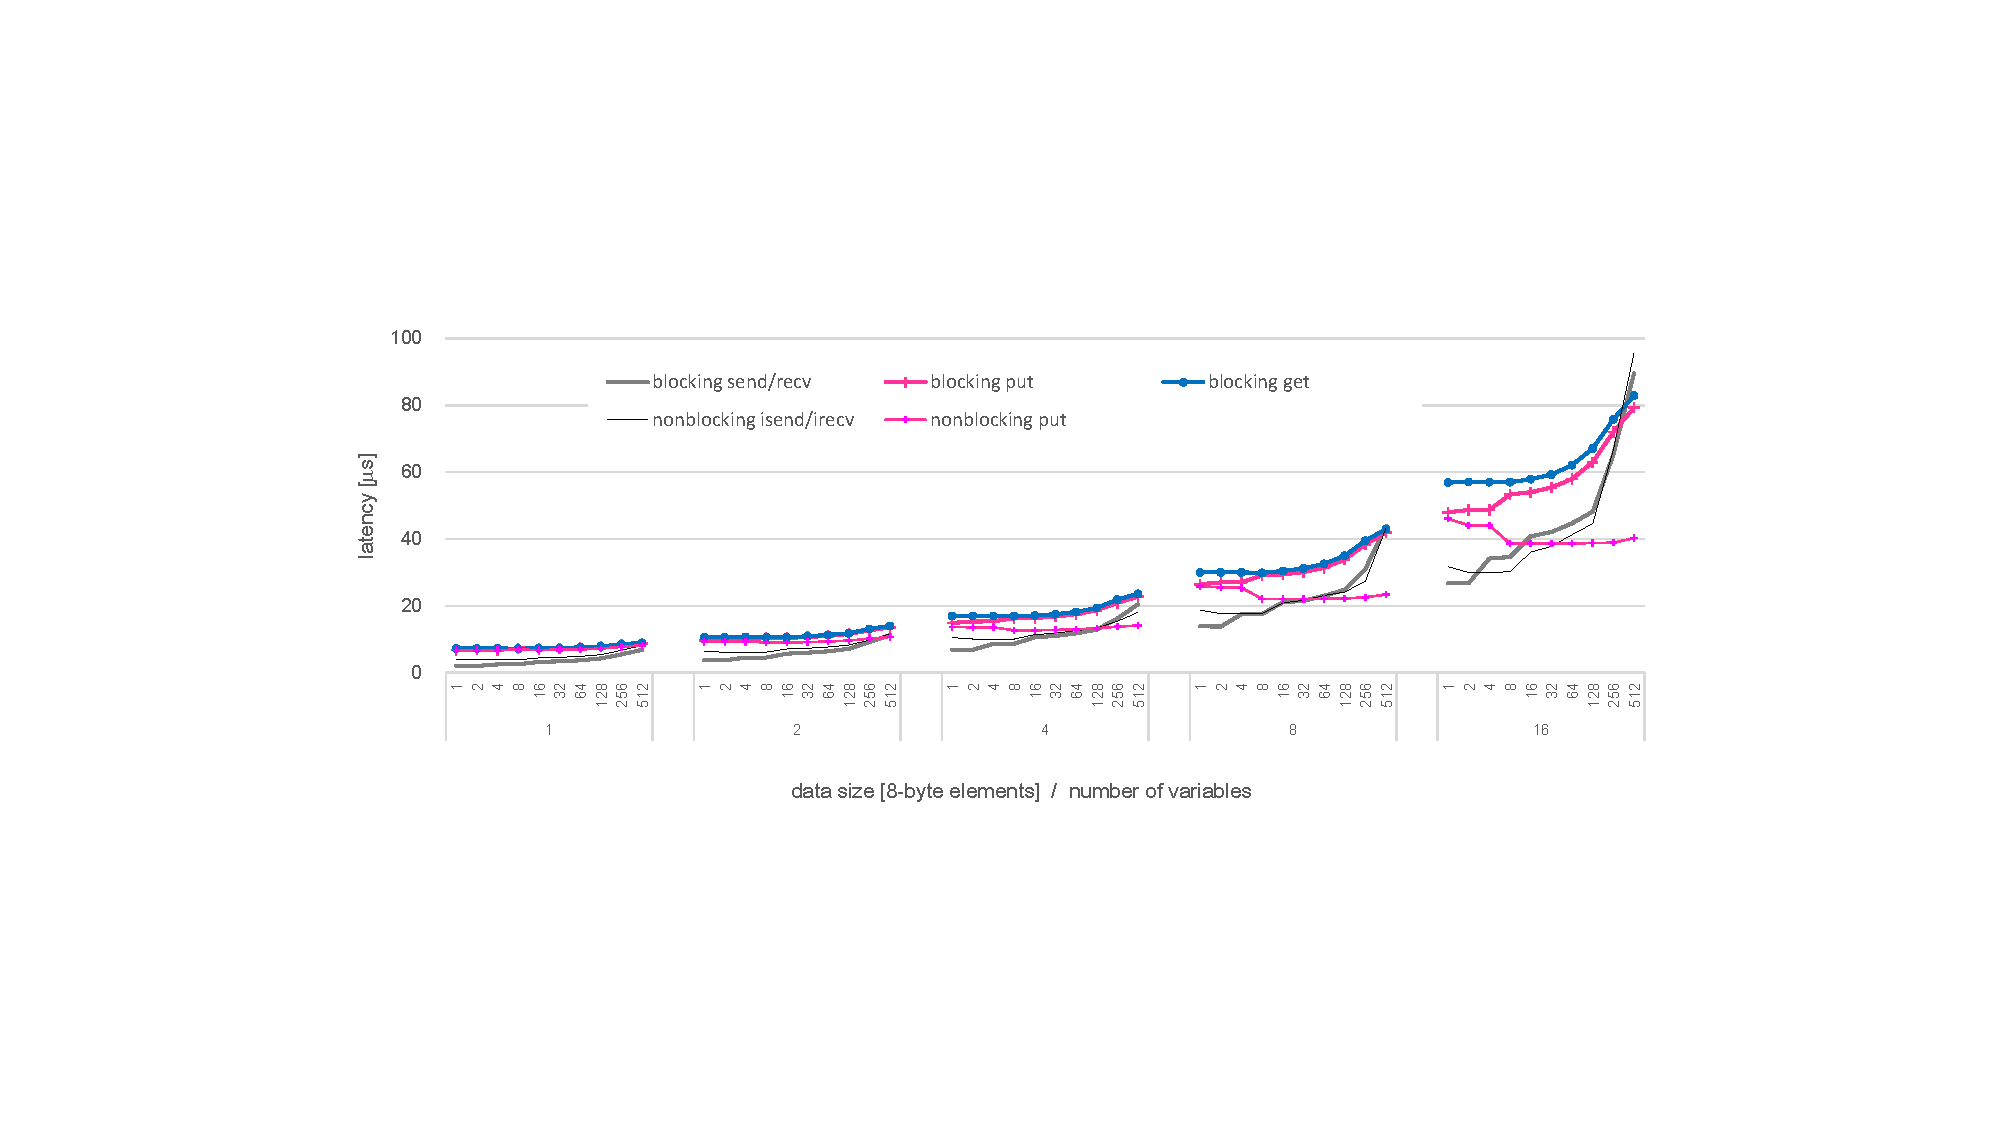
\includegraphics[scale=0.55,trim=6cm 0cm 4cm 6cm,clip]{figs/latency-16var.pdf}

  latency-16var.pdf\\
  2からの4つにして図を大きくする。
  \caption{n-var latency of pingpong}\label{fig:nvar-pp}
  \end{center}
\end{figure}

n-varの効果があった。実際のアプリでもこれはよく起こるパターンである。


\begin{figure}[tbh]
  \begin{center}
  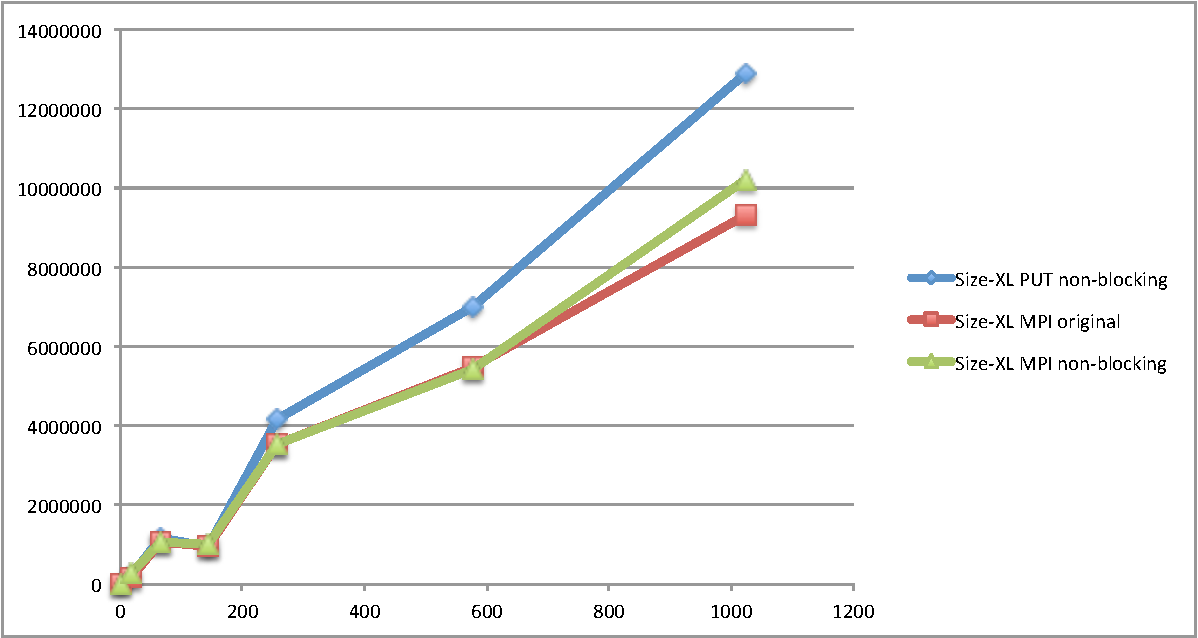
\includegraphics[scale=0.55]{figs/himeno.pdf}

  棒グラフにしてLを加えて2つにするかMまで加えて3つにする

  cf.\ air:/Users/iwashita/Desktop/coarray/Project\_Coarray/coarray\_runtime.pdf

  \caption{Himeno XL}\label{fig:himeno}
  \end{center}
\end{figure}


どういうパターンか分析して説明。n個のcontiguousなnonblocking comm.


\subsection{OTHERS}


%-- 3cell-y.pdf
%-- 3cell-z.pdf
\begin{figure}[tbh]
  \begin{center}
  % trimはleft bottom right topの順
  \fbox{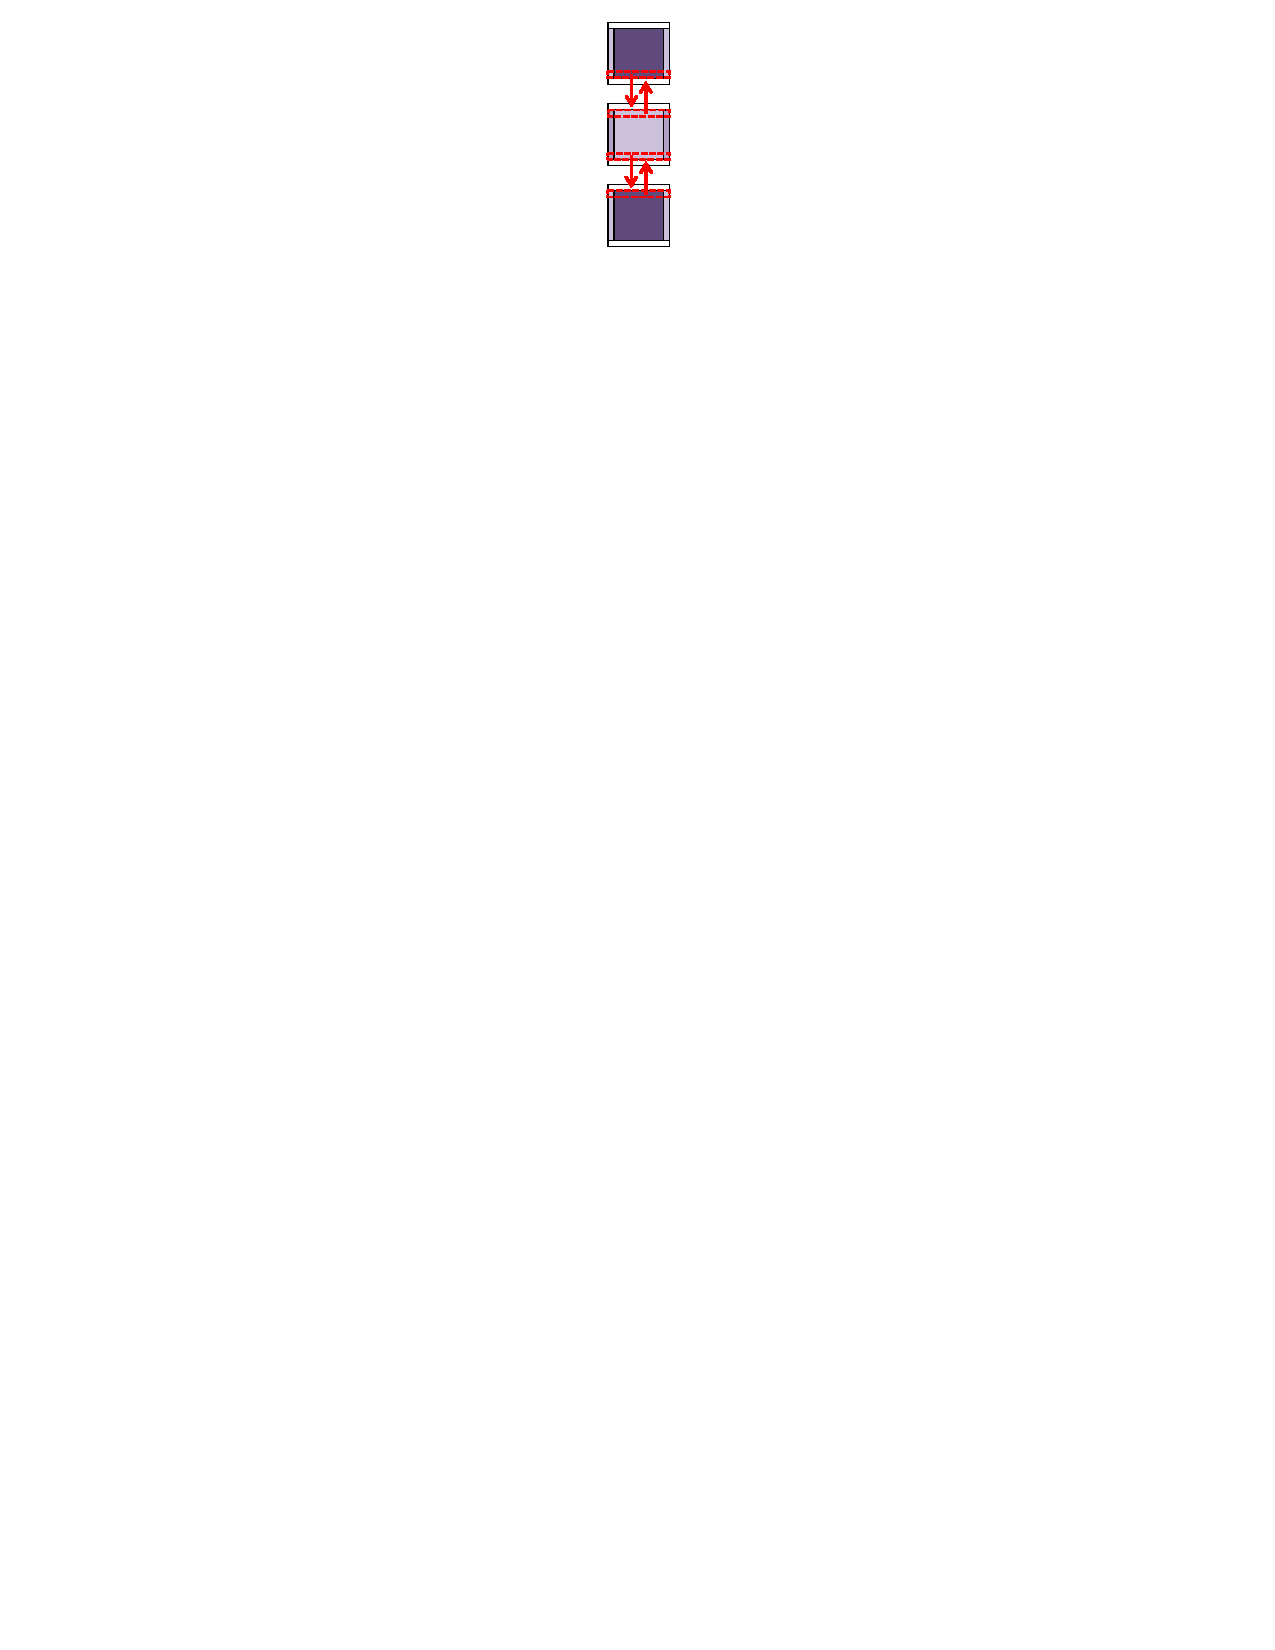
\includegraphics[trim=98mm 235mm 98mm 0mm, scale=0.8,clip]{figs/3cell-y.pdf}}  \\
  \fbox{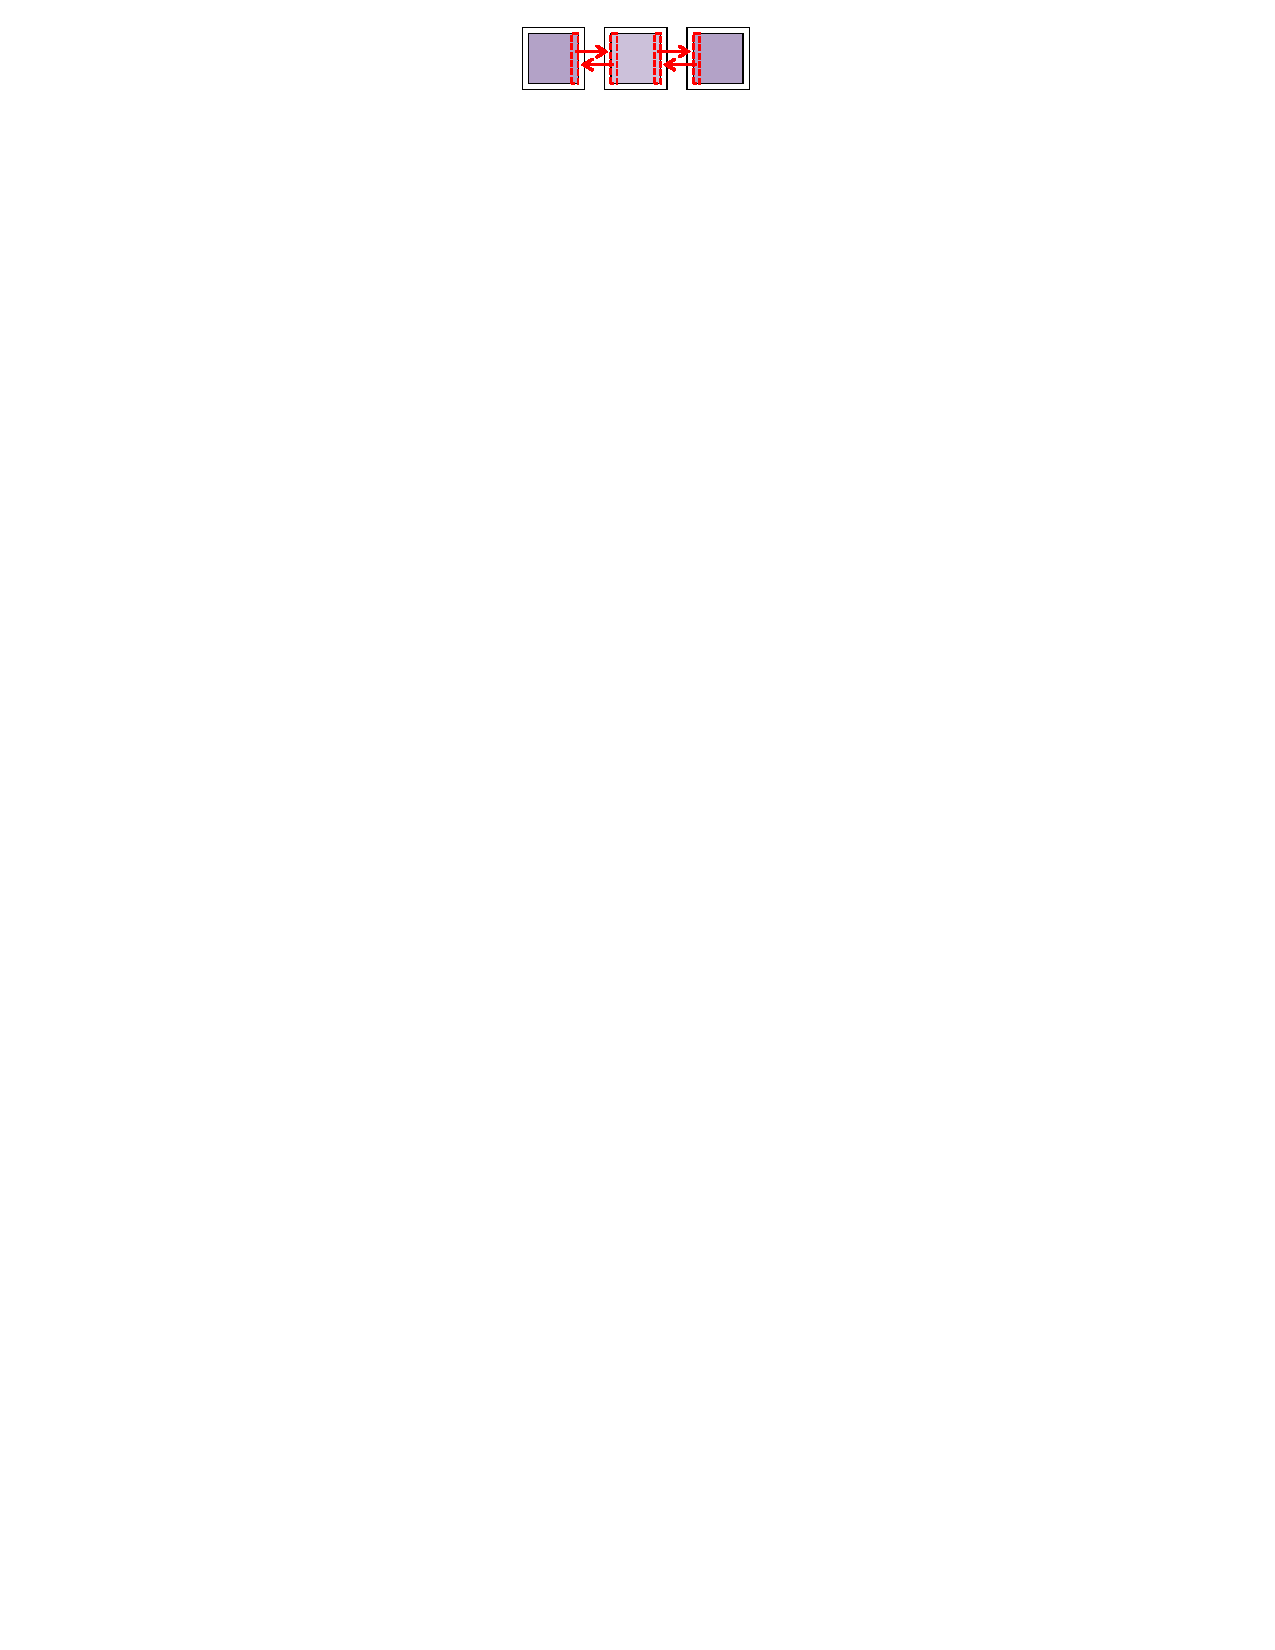
\includegraphics[trim=85mm 261mm 85mm 0mm, scale=0.8,clip]{figs/3cell-z.pdf}}  \\
  \fbox{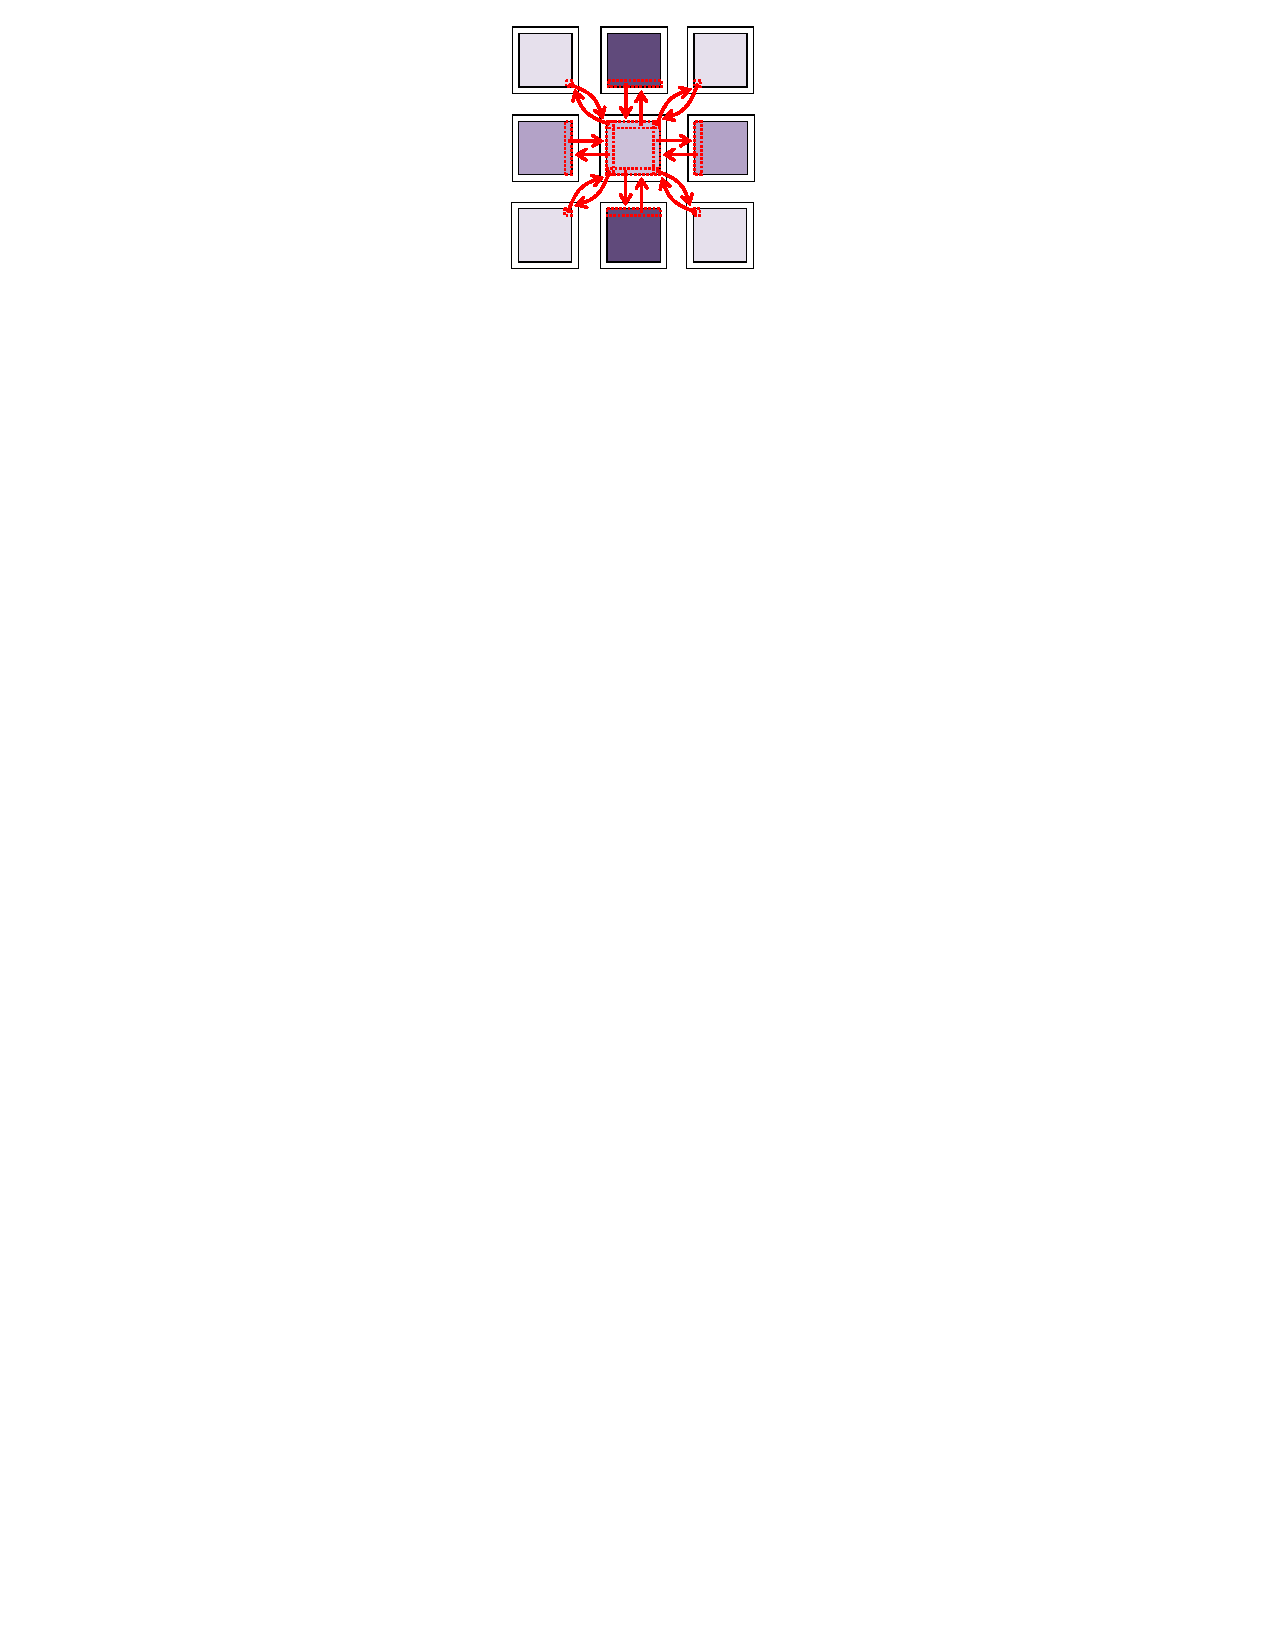
\includegraphics[trim=82mm 230mm 84mm 0mm, scale=0.8,clip]{figs/9cell-yz.pdf}}
  \caption{3cell-y.pdf, 3cell-z.pdf, 9cell-yz.pdf}\label{fig:cell}
  \end{center}
\end{figure}


%-- 8var-pipo-latency.pdf
\begin{figure}[tbh]
  \begin{center}
  % trimはleft bottom right topの順
    \fbox{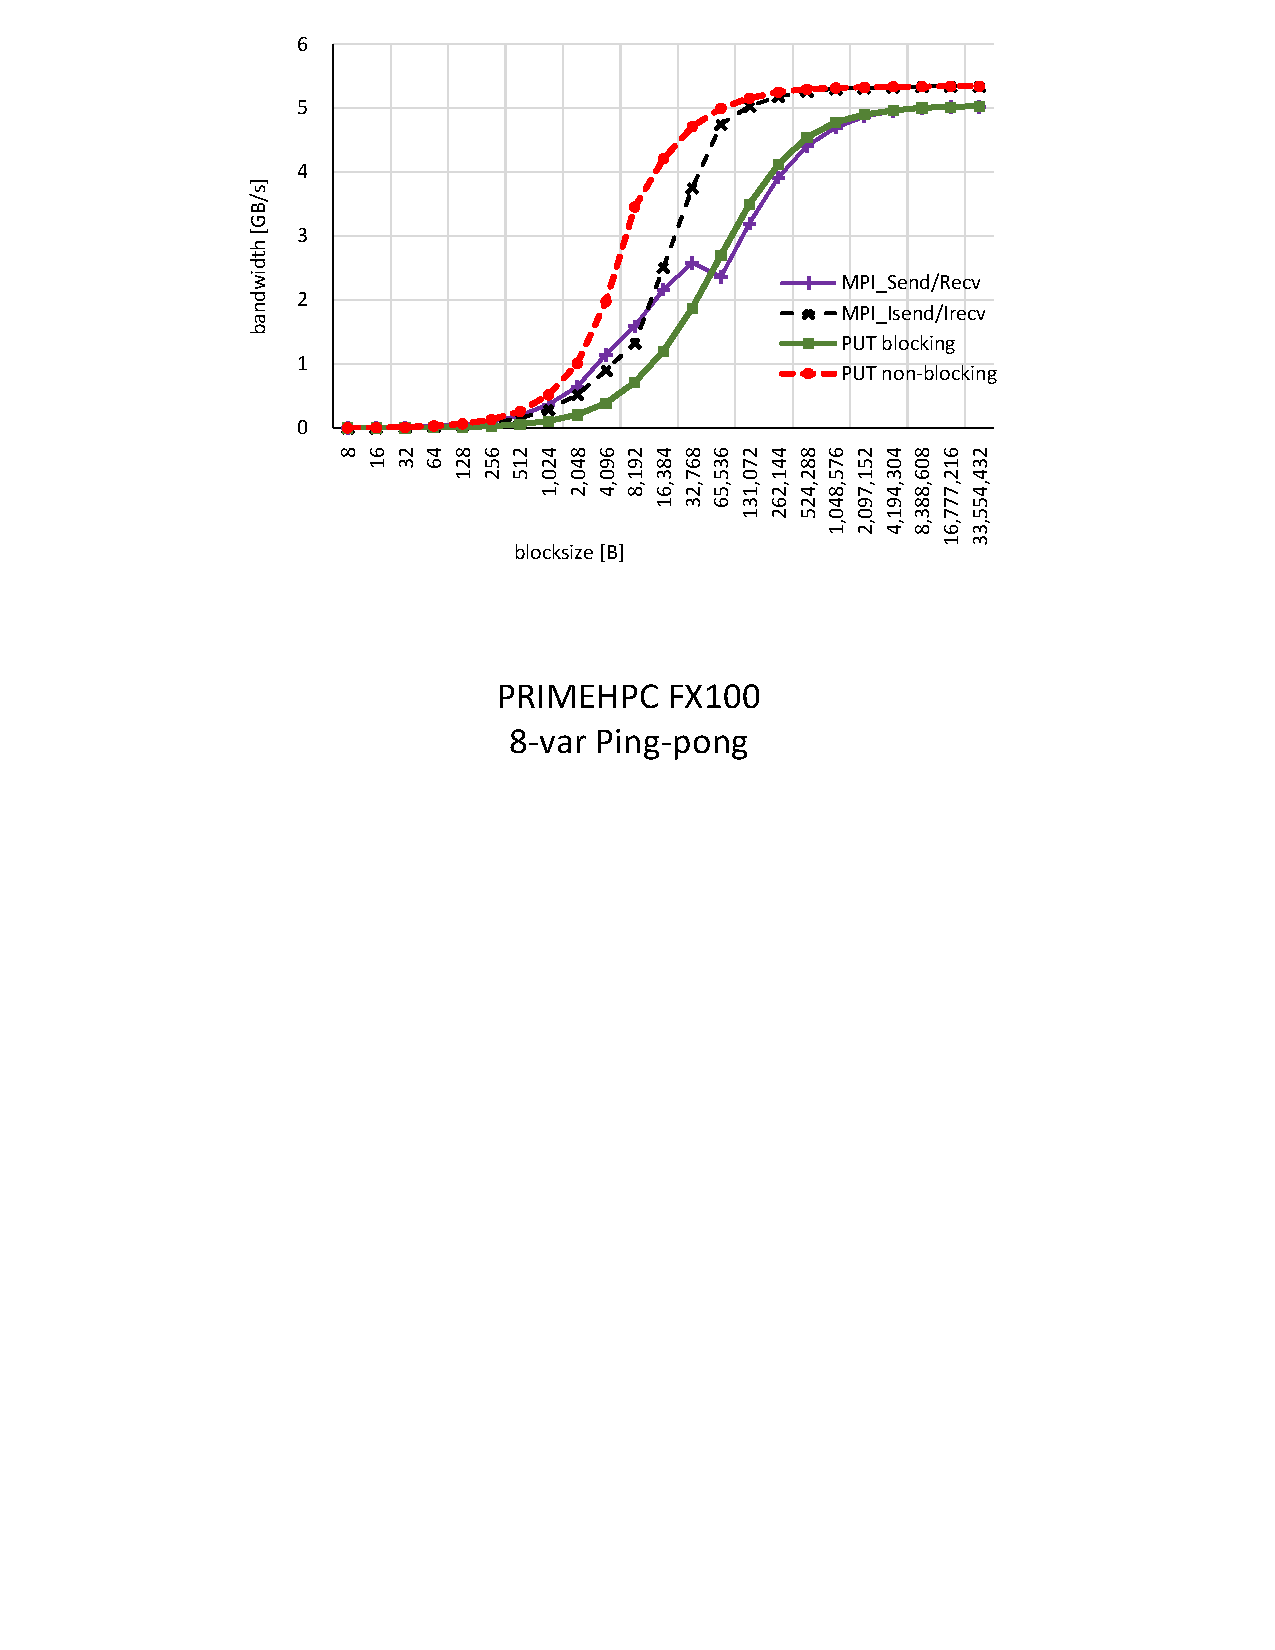
\includegraphics[trim=40mm 180mm 43mm 0mm, scale=0.8,clip]{figs/8var-pipo-bw.pdf}}
    \caption{8var-pipo-bw.pdf}\label{fig:8var-pipo-bw}
  \end{center}
\end{figure}

%-- 8var-pipo-latency.pdf
\begin{figure}[tbh]
  \begin{center}
  % trimはleft bottom right topの順
    \fbox{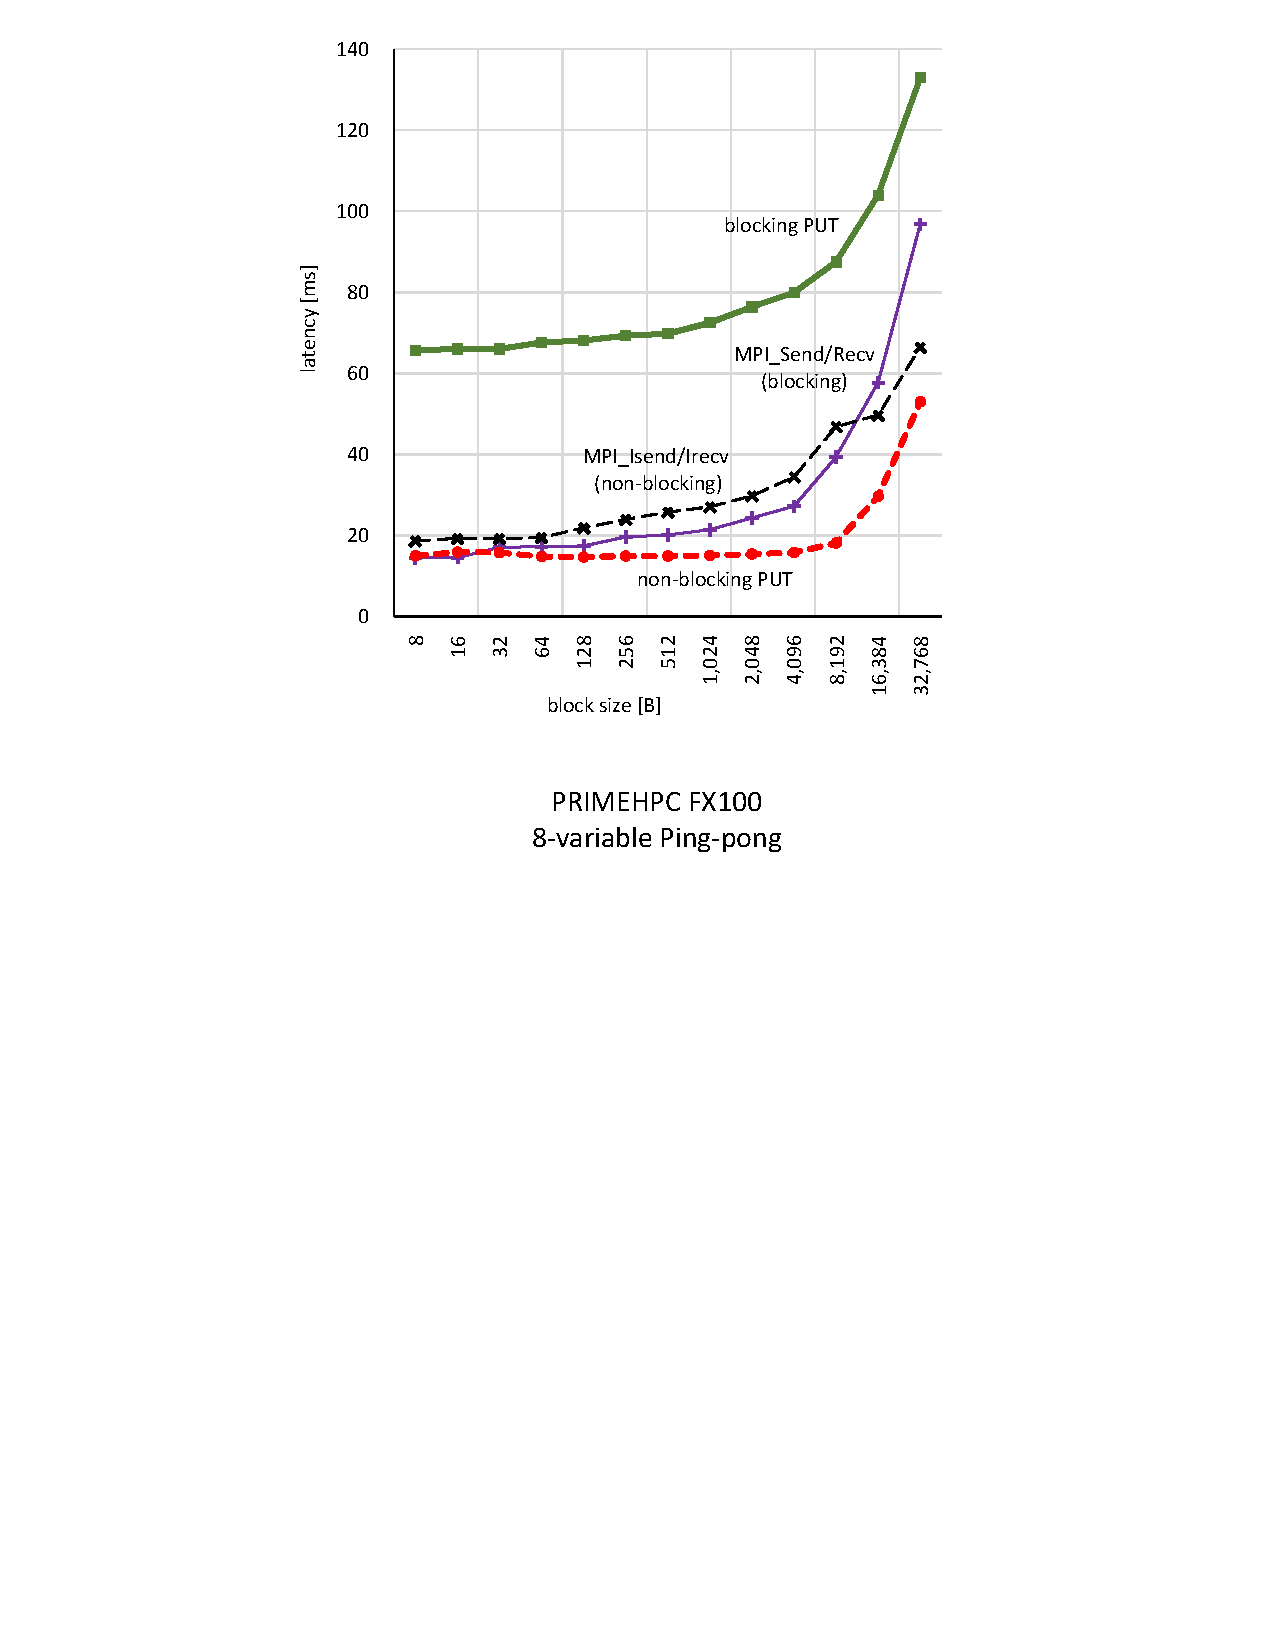
\includegraphics[trim=40mm 155mm 40mm 0mm, scale=0.8,clip]{figs/8var-pipo-latency.pdf}}
    \caption{8var-pipo-latency.pdf}\label{fig:8var-pipo-latency}
  \end{center}
\end{figure}

%-- HAPACS-bw.pdf
\begin{figure}[tbh]
  \begin{center}
  % trimはleft bottom right topの順
    \fbox{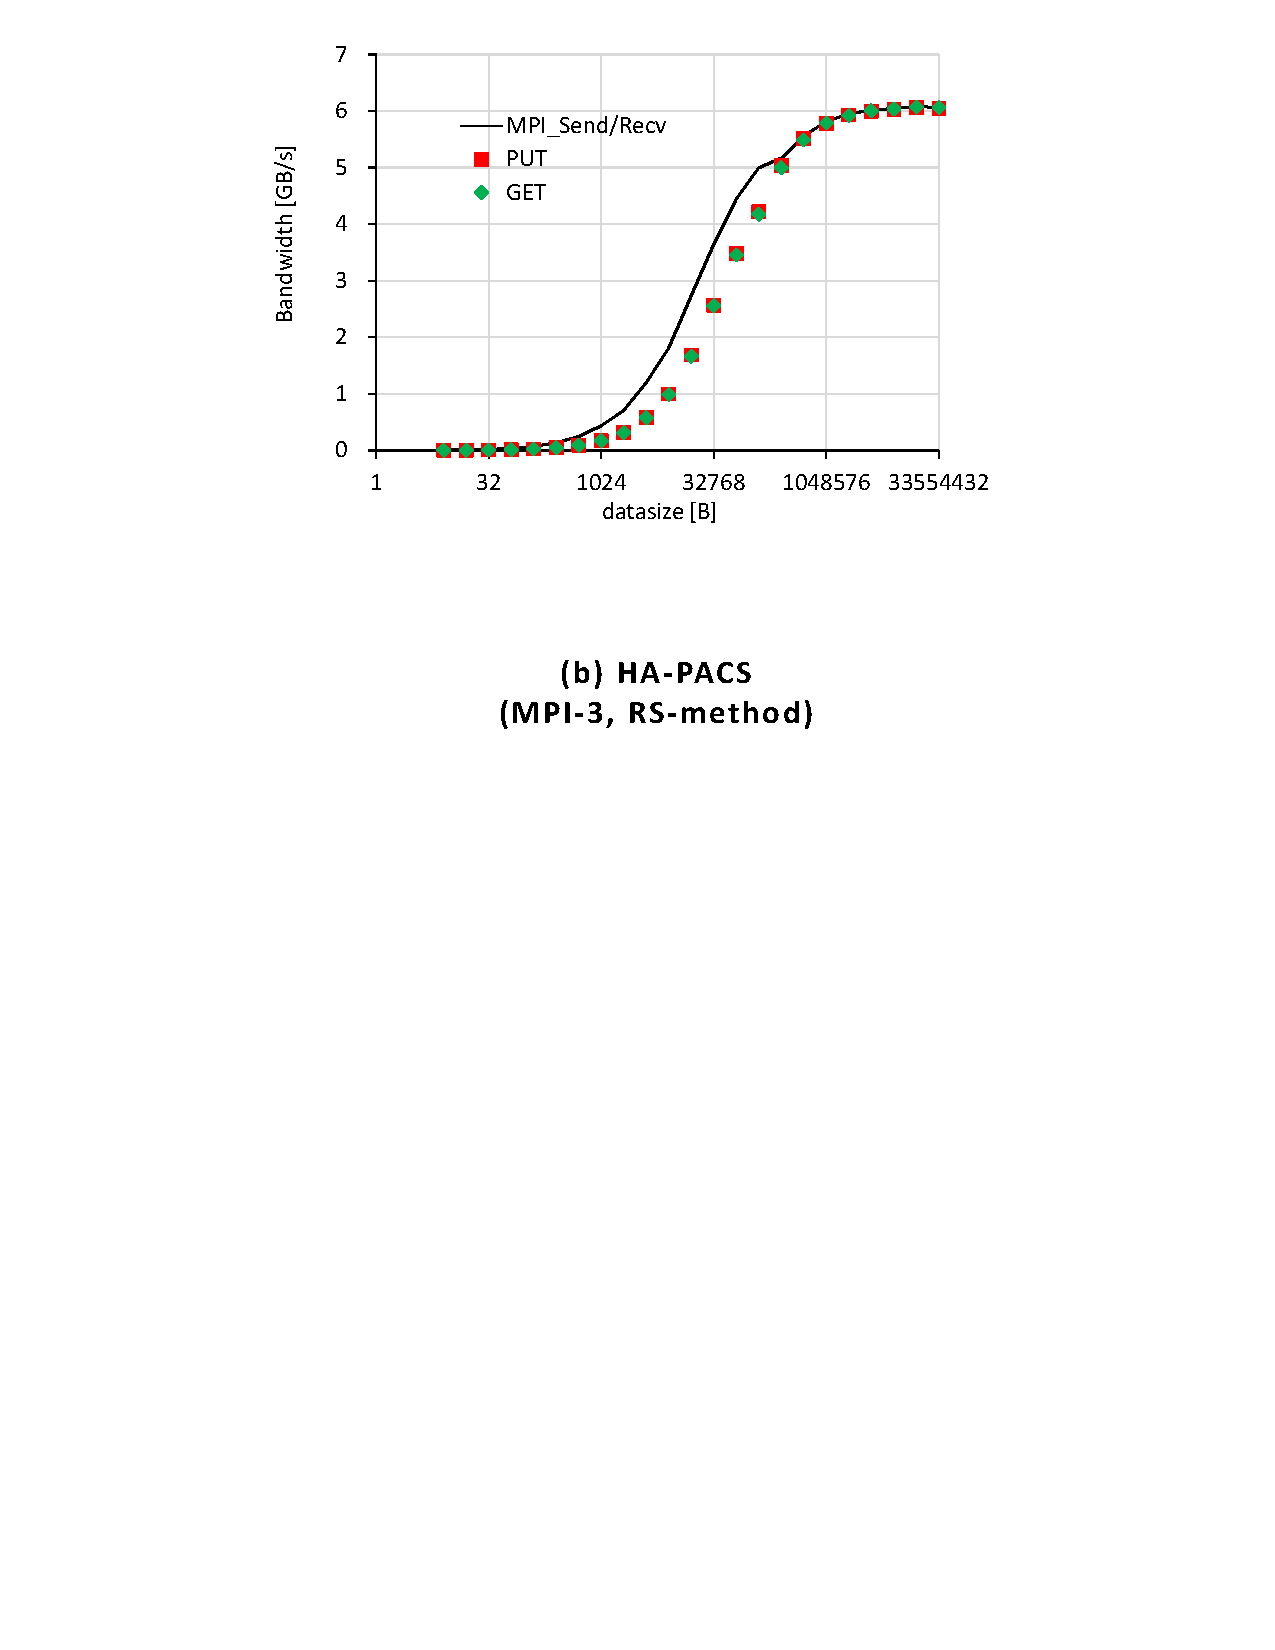
\includegraphics[trim=45mm 188mm 45mm 3mm, scale=0.8,clip]{figs/HAPACS-bw.pdf}}
    \caption{HAPACS-bw.pdf}\label{fig:HAPACS-bw}
  \end{center}
\end{figure}

%-- fx100-bw.pdf
\begin{figure}[tbh]
  \begin{center}
  % trimはleft bottom right topの順
    \fbox{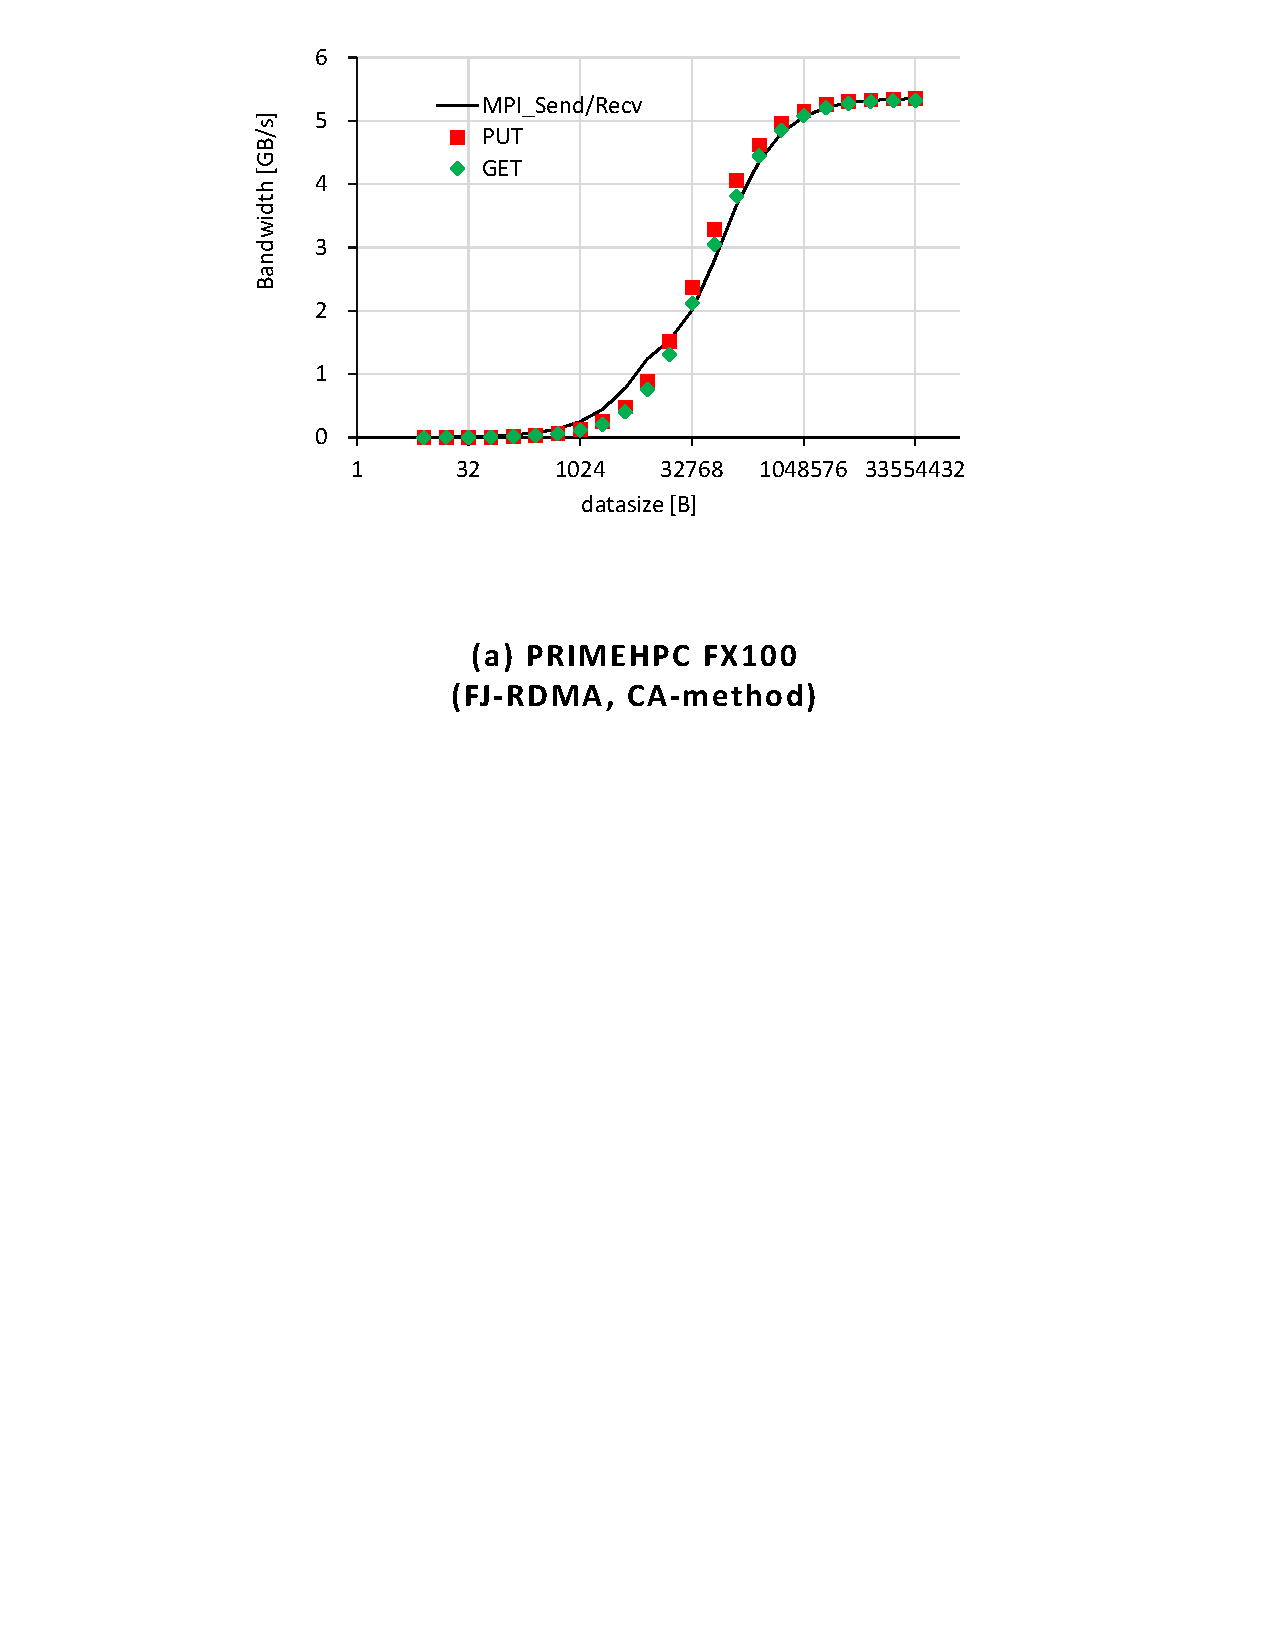
\includegraphics[trim=41mm 190mm 49mm 3mm, scale=0.8,clip]{figs/fx100-bw.pdf}}
    \caption{fx100-bw.pdf}\label{fig:fx100-bw}
  \end{center}
\end{figure}

%-- fx100-pipo.pdf
\begin{figure}[tbh]
  \begin{center}
    % trimはleft bottom right topの順
    \fbox{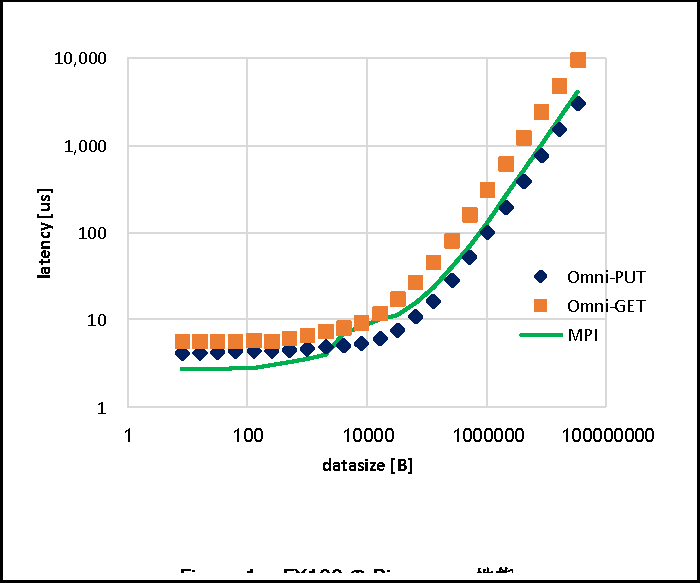
\includegraphics[trim=4mm 15mm 4mm 3mm, scale=0.9,clip]{figs/fx100-pipo.pdf}}
    \caption{fx100-pipo.pdf}\label{fig:fx100-pipo}
  \end{center}
\end{figure}

%-- himeno-K-nonblock.pdf
\begin{figure}[p]
  \begin{center}
  % trimはleft bottom right topの順
    \fbox{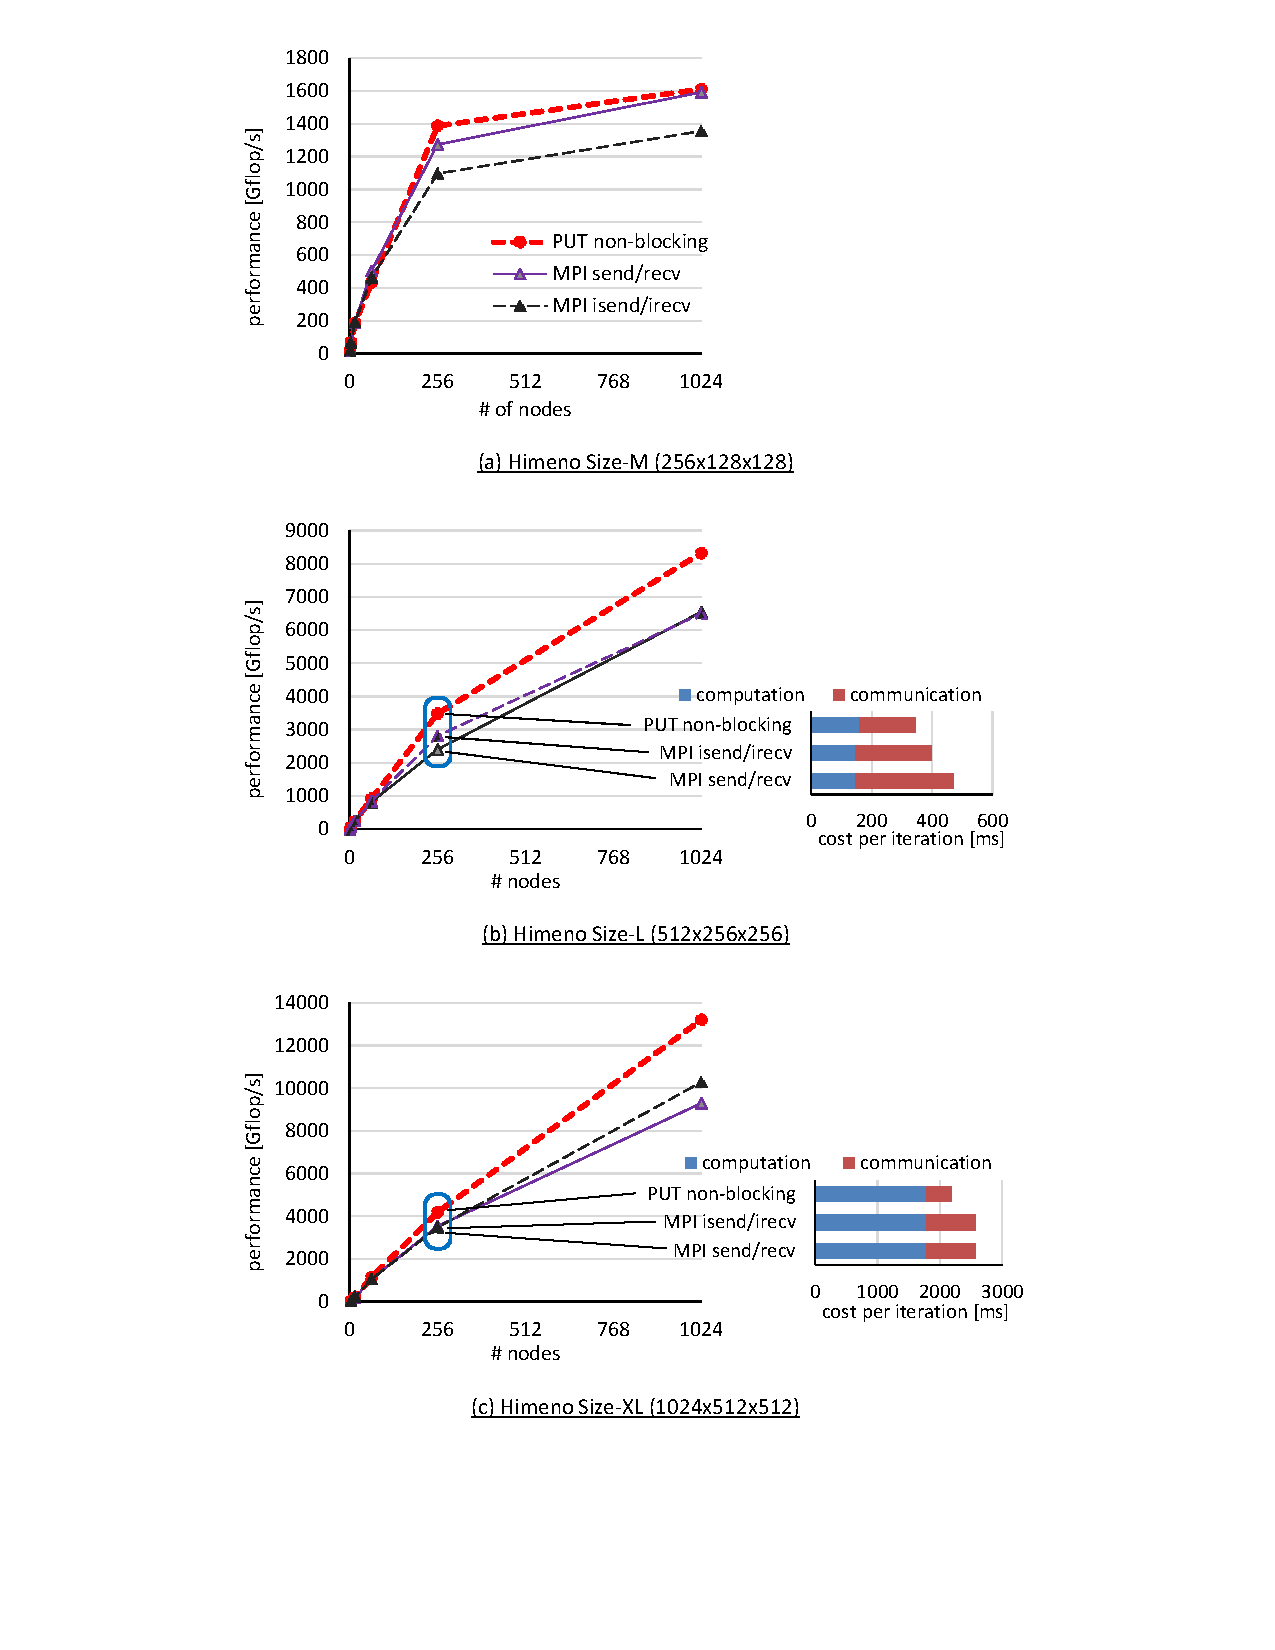
\includegraphics[trim=37mm 34mm 37mm 4mm, scale=0.8,clip]{figs/himeno-K-nonblock.pdf}}
    \caption{himeno-K-nonblock.pdf}\label{fig:himeno-K-nonblock}
  \end{center}
\end{figure}

%himeno.pdf
%latency-16var.pdf
%layer.pdf
%-- nonblock-fig.pdf
\begin{figure}[tbh]
  \begin{center}
  % trimはleft bottom right topの順
    \fbox{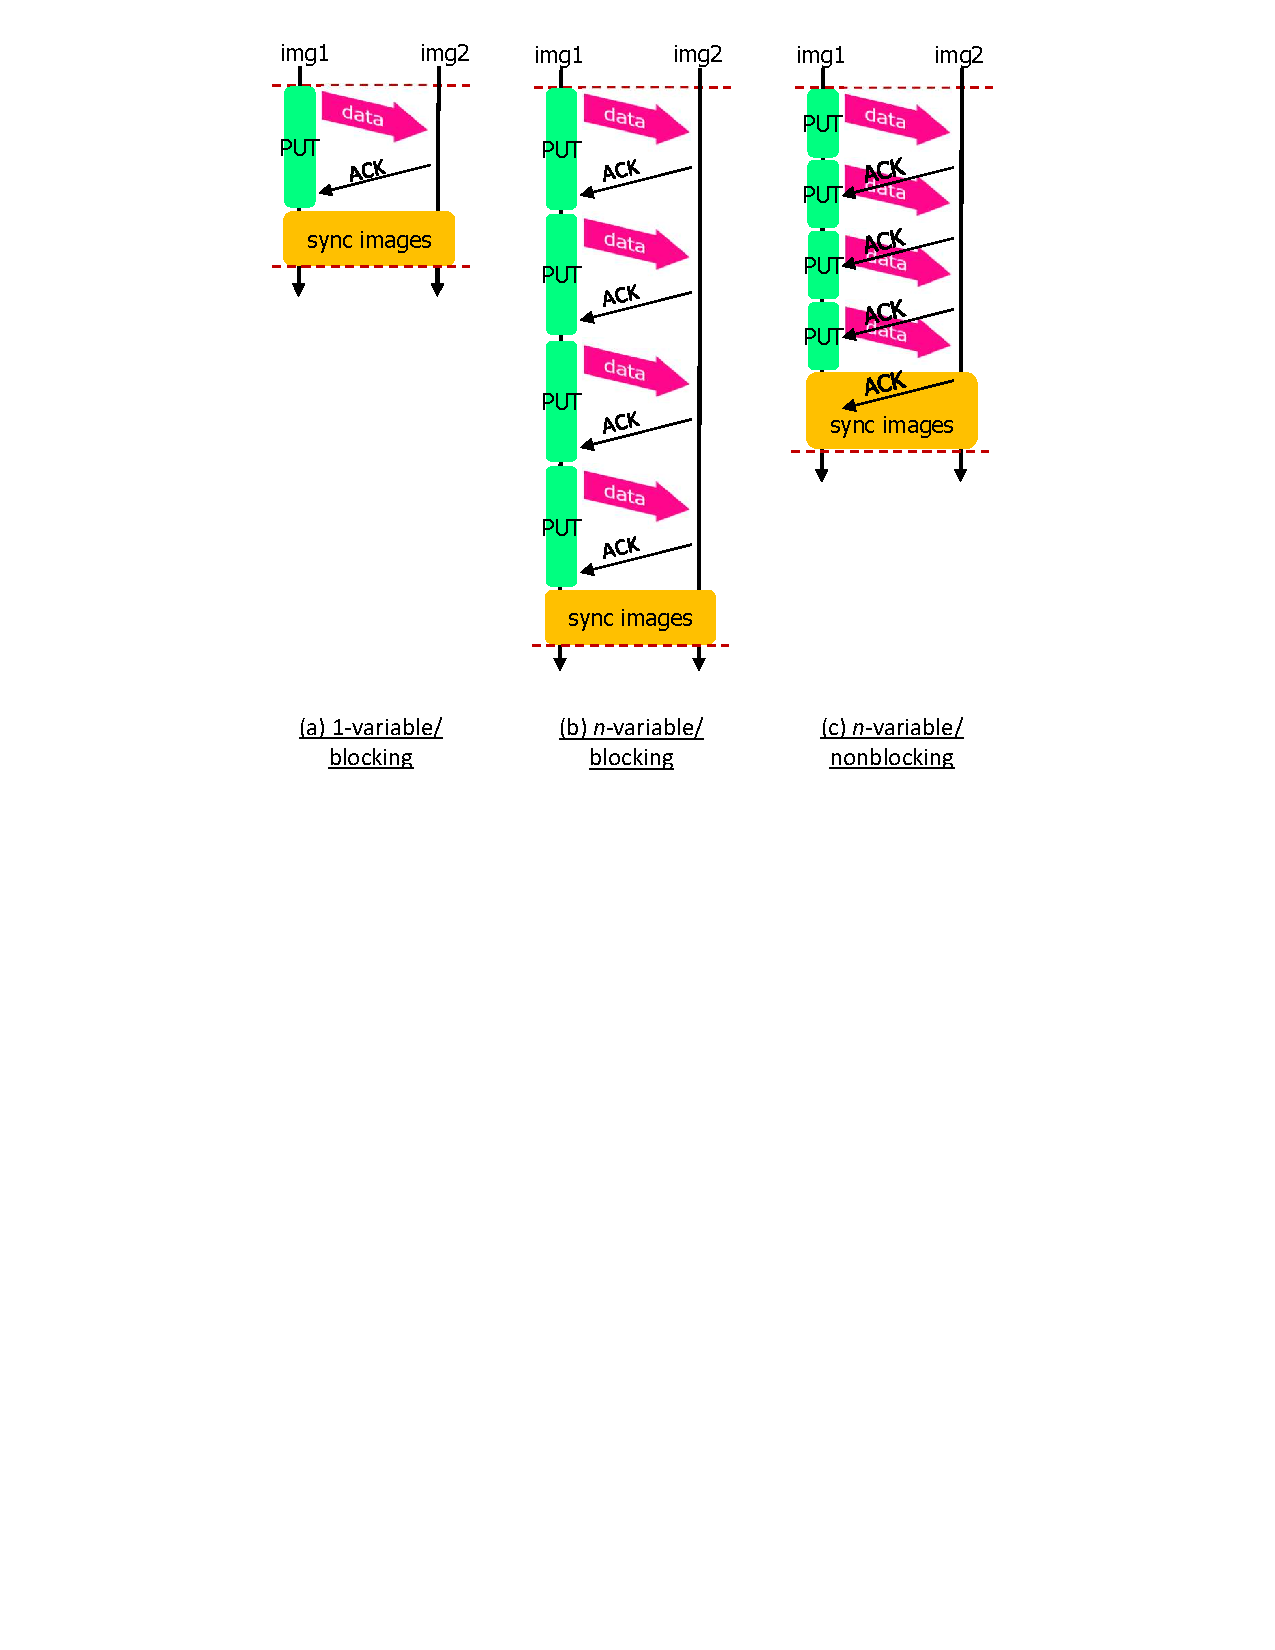
\includegraphics[trim=43mm 144mm 43mm 3mm, scale=0.8,clip]{figs/nonblock-fig.pdf}}
    \caption{nonblock-fig.pdf}\label{fig:nonblock-fig}
  \end{center}
\end{figure}

%-- pingpong-code.pdf
\begin{figure}[tbh]
  \begin{center}
  % trimはleft bottom right topの順
    \fbox{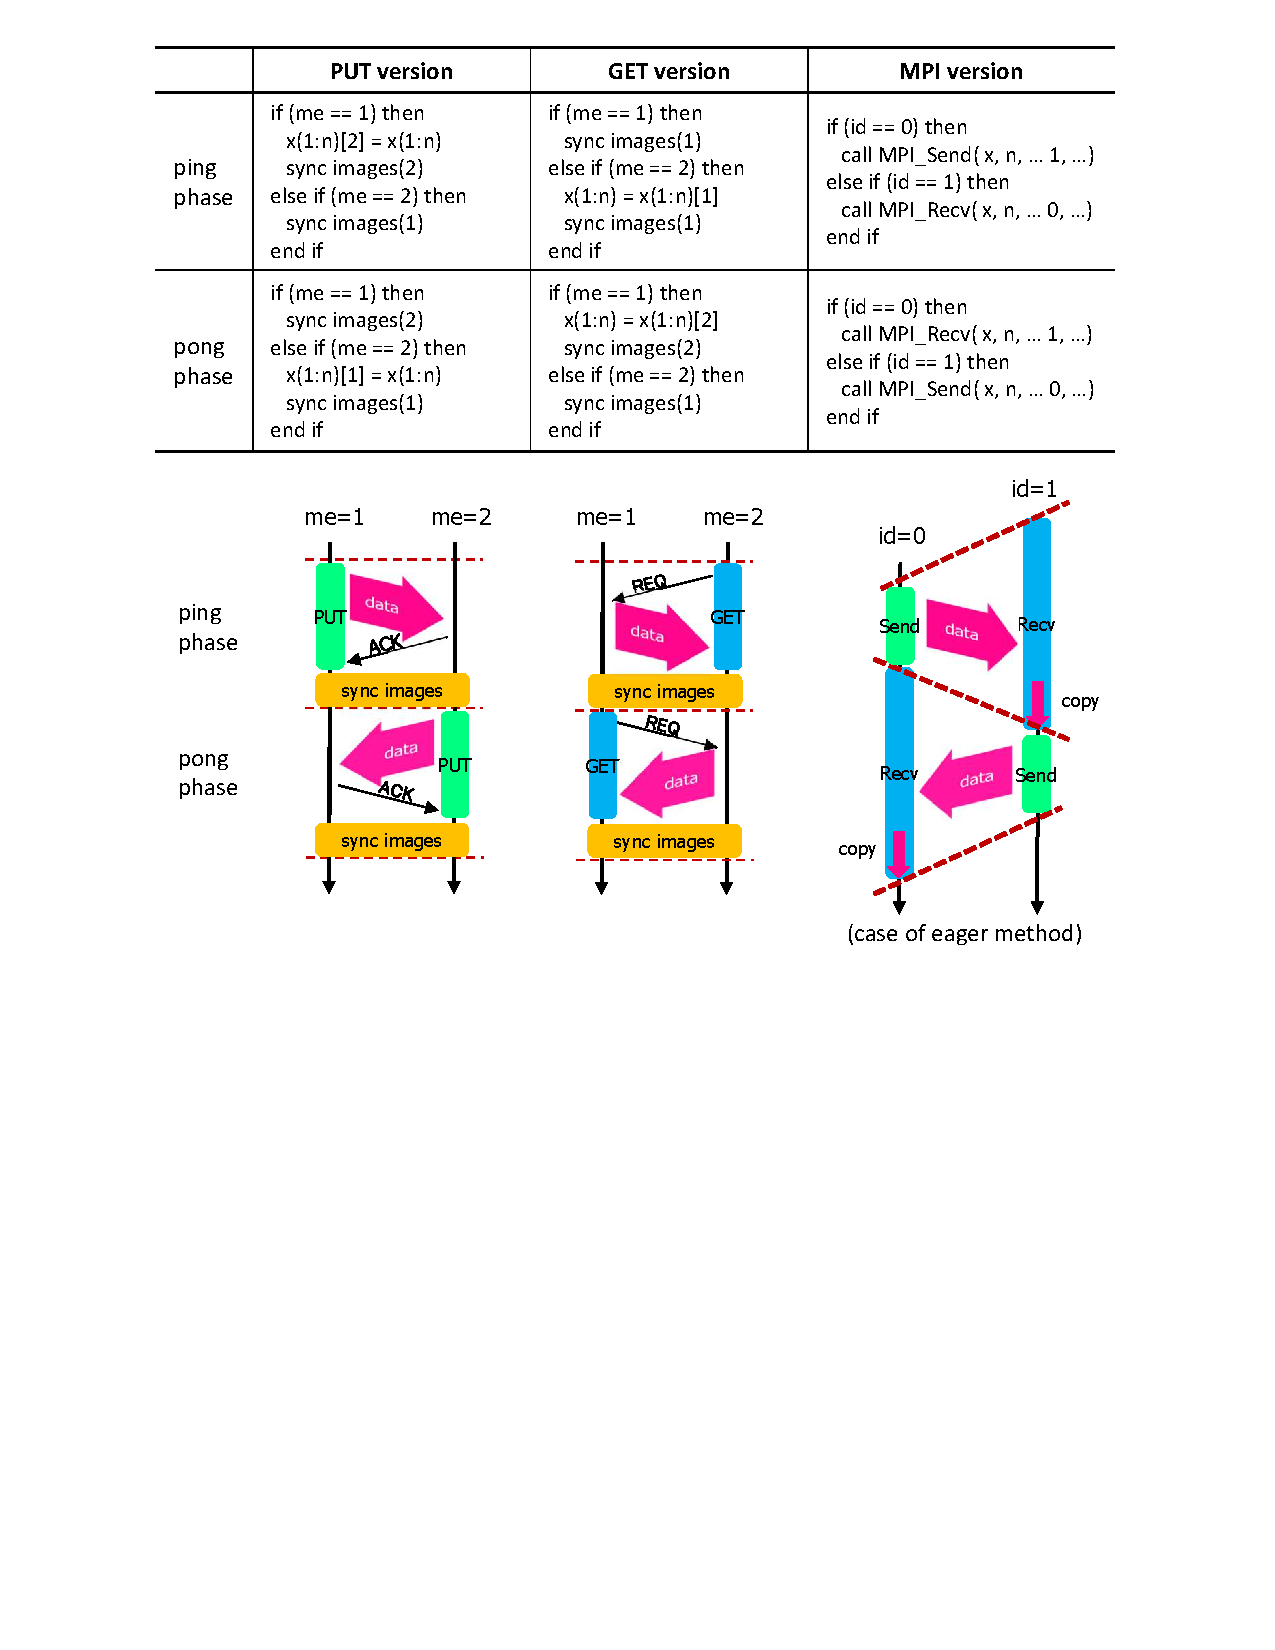
\includegraphics[trim=24mm 118mm 24mm 4mm, scale=0.7,clip]{figs/pingpong-code.pdf}}
    \caption{pingpong-code.pdf}\label{fig:pingpong-code}
  \end{center}
\end{figure}

%register-CA-tmp.pdf
%register-RA-CA-tmp.pdf
%register-RA-tmp.pdf
%softstack.pdf
%translator-tmp.pdf
